\chapter{Introduction}

\section{Problem}
(Could I just say models, here instead of generative models?)
\begin{itemize}
  \item Real world data if often causesed by multiple sources, that is independant sources combining to form data.  This creates noise and obscures part of the data we are interested in.
  \item Generative Models used in Machine learning do not capture these source independantly, meaning prior knowledge about the data is being lost(To much of a sweeping statement?). Instead the generative models are trained to learn the complex combination of data caused by the sources.
  \item Generative Model that do account for multiple sources are desirable, as the causes are encoded separately, which would(should this just be allows?) allow source separation. That is, taking a noisy input and encoding that into separate representations for each source.
  \item When the model treats sources naively, more work on data preprocessing and cleaning is needed, which often takes longer that the machine learning task itself.
  \item Frean, Marsland propose a new Generative Model that can capture two causes combining to form data, effectively encoding prior knowlege into the architecture of the model.
  \begin{itemize}
    \item It builds on and combines previous work on Restricted Boltzmann Machines and Sigmoid Belief Networks.
    \item The theory had been checked but the new model had not been tried in practice. Frean and Marsland needed confidence around some key areas
    \begin{itemize}
      \item Can this model encode a multi-cause input(need to define this?) as separate causes? That is, can the model be used to perform source separation. Given this produces an internal representation, how can we evaluate whether or not is it working?
      \item How does the time-efficiency of this model compare to the standard Restricted Boltzmann machine? The architecture of the new generative model has a richer structure. The theory shows that the new approach has the potential to be slower than an RBM to generate a hidden representation. Is this an issue in practice?
    \end{itemize}
    \item These are non-trivial tasks as the Restricted Boltzmann Machine, and the proposed model that uses it, are stochastic unsupervised learners making evaluation non-trivial. We cannot simply inspect the representations generated in the new model.
    \item There is(was?) a need to implement this new approach and then verify that it can or cannot perform source separation.
  \end{itemize}
  \item In addition to the new algorithm Two approximations that allow the algorithm
  more efficient need to be evaluated and compared to the full approximation.
\end{itemize}

\section{Solution}\label{Sec:Intro:Solution}

\begin{itemize}
  \item This project answered(answers?) these questions, evaluating the new generative model by way of experimentation. The ablility for the new generative model (I really need a name for this)  to separate the sources has been evaluated on various sizes (better word here) of problems.
  \item The unsupervised nature of the new model and the models it builds on, are non-trivial to evaluate. To explain the evaluation techniques and the new model itself some concepts/terminology must first be introduced.
\end{itemize}

\section{A Concrete Scope}

As the theory already had the Mathematical ground work by Frean and Marsland the scope of this project is not to prove the theory mathematically, instead impelmenting the Algorithm and verfiying how it behaves in practice by answering the questions posed in \ref{Sec:Intro:Solution}.

\chapter{Background}

\section{Context}

\subsection{Source Separation}

\begin{itemize}
  \item Introduce the idea of data with mutiple sources, probably by way of the cocktail party problem like in prelim.
  \item Go on to reference previous work in Source separation to show the importance/interest in the area. 5 Papers should suffice.
\end{itemize}

\subsection{Probablistic Graphical Models}

Probalistic Graphical Models or PGMs for short, are an expressive way to represent a collection of stochastic  variables. If the graph is directed then the edges represent causation, this is also referred to a Bayesian network. Conversely, if the graph was undirected then edges represent a mapping. TODO-CITE-DAVID-BARBERS-TEXTBOOK-ON-PGM-USE.

\subsection{Generative Models}

Generative models are a powerful way to model data. (TODO-GRAB-THOSE-GENERATIVE-MODEL-USES-CITATIONS)

In the context of images, generative models, if trained, can randomly generate observable data. (Don't like the wording of this)
The generative model proposed in this project aims to represent data generated by two causes.

  \subsubsection{Observable and Hidden Variables}

  \begin{itemize}
    \item Describe how the models have some latent factors/variables that represent the cause, or an efficient encoding/representation of the data we want to learn.
    \item Make sure to describe/define analogus terms like hidden visible layers, variables/units etc.
  \end{itemize}

  \subsubsection{Training Generative Models}
  \begin{itemize}
    \item Training generative models with some param big theta, gradient amounts to log likelihood of dataset minus normalisation.
    \item Amounts to hebbain learning. Reasoned about by Donald Hebb, connections between neurons in the brain during learning, the more often a memory is accessed or used, the strong the connection it should make. Nice to have parallels with biology. Something biology performs well that Machine learning has difficulty with is source separation.
    \item Wake phase - Often referred to as the clamped phase of training involves clamping the input of the model to a data item and trying to increase that items probability. Essentially this amounts to building probabilty mass around the items in the training set.
    \item Sleep phase - Also referred to as the free phase, this acts as complexity control where the the generative model is used to create data items...
    \item Quickly talk about the learning rule
  \end{itemize}

\subsection{Sampling}

Sampling is the process of drawing samples from a distribution. It is used when the distrubtion we want samples from is intractable to calculate analytically. Sampling is required to train generative models, as often the gradient to be climbed/descended involves calculating a probability in the
generative model.

\begin{itemize}
  \item Inference is the process of given reasoning about what we do not know given that of which we do know.
  \item In a Generative Model this amounts to the Posterior
\end{itemize}

  \subsubsection{Markov Chain}

  \begin{itemize}
    \item The importance of Markov Chains and mixing time are crutial in this project
  \end{itemize}


  \subsubsection{Gibbs Sampling}

  Gibbs sampling is a special case of Markov Chain Monte Carlo, a technique for sampling from a complex distribution. The probability mass of a generative model is a common use case for Gibbs sampling.

  \subsubsection{Reconstructions}

  Generative Models can create an internal representation given an input. They can also generate a faux input given an internal representation. Performing one Gibbs iteration, that is sampling from the hidden units given an input $ P(h|v) $ and then taking the generated hidden state and generating a faux input. The model tries to reconstruct the input.

  \subsubsection{Fanstasies of the Model}

  In the same way that a generative model uses reconstructions to try and recreate the      supplied input based purely on how it's represented that input, performing many, many (greater than 100) Gibbs iterations with no input pattern clamped allows the reconstructions to explore the probability mass that the model has built up during training. Sampling from these wanderings creates what are refferred to as 'fantasies' or 'dreams'. These give a sense of what the model has learnt, and can act a smoke test for if the model has actually capture anything.
  (TODO-CITE-PAPER-WITH-MNIST-DREAM-EVALUATION, they were crappy).

\section{An Intractable Model For Causes}
  \subsection{Belief Networks}

  A belief network is technique(? Graphical Network ?) of modeling causual data. The network is directed representing cause, nodes in the network represent binary variables which are dependant on ancestor nodes, the degree of which is encoded in a conditional probalitity table. The belief network provides a succint encoding of depedancies between variables. Several algorithms operate on this representation, determining the probability of a variables state, given the states of its ancestors. One of such algorithms is Belief Propagation/Sum-Product Algorithm. However this technique breaks down in larger dimensions with a cost of TODO


  The technique proposed in this report relies on the parameterised version of the belief network, the Sigmoid Belief Network. The sigmoid belief network is composed of sigmoid units, akin to that of a perceptron linear threshold unit. The weighted sum of the inputs to a variable in the system is passed through a sigmoid function, the weights capturing the dependance between a node and its ancestors.

  Belief Networks appear to be an intuitive way to model data in machine learning, as rich dependancies often present in real data can be expressed in its architecture. Unfortunately, due to the effect of explaining away, it is intractable to perform inference in a belief network which is needed required for training.

  \subsection{Explaining Away}

  The power of the belief network is also its weakness, a rich structure that models a system of interest inheriently has depedancies. In its minimal case explaining away can be seen in a 3 node network popularised by TODO-CITE-AI-A-MODERN-APPROACH-TODO. TODO-GRAPHIC

  In this network knowledge of the alarm creates a dependance between Burglar and Earthqaukes. For instance, say the Alarm has gone off and we know an earthquake has occurred, our belief in being burgaled decreases. The dependance in belief networks means that sampling from the network requires a longer Markov Chain to mix.

  In the context of images, where there may be upwards of 1000 observable values, all with different depedancies this is intractable.

\subsection{Boltzmann Machines}

A Boltzmann machine shares a few qualities with Belief Networks. Both are generative models, and variables/nodes have probabilities of being active/deactive based on neighbouring nodes. Unlike a Belief Network, a Boltzmann Machine is a undirected network meaning connections between nodes no longer encode causal information. Performing gibbs sampling appears trivial in a Boltzmann Machine, in that to find the probability of a given unit being active a weighted input to that node is passed through a sigmoid function. However, in practice the recurrent nature of Boltzmann Machines makes sampling intractable.

TODO-REFENCE-PAPER-OF-THIS The Boltzmann Machine was shown, given an unreasonable amount of time, to be able to perform better than the state of the art at the time.

\section{The Current Approach: A Strong assumption}

\subsection{Restricted Boltzmann Machines}

Hinton TODO-REFERENCE-THE-PAPER proposed a restriction by way of assumption to the Boltzmann Machine that makes it tractable to sample from and therefore train. Boltzmann Machines of this architecture are referred to as Restricted Boltzmann Machines, or RBMs for short.

The assumption being that the observable and latent variables are independant respectively, enforcing a two layer, fully connected bipartide structure. The affect of this being that inference can be tractably computed as the latent variables no longer become dependant given the observed variables.

  \subsubsection{Tractable Training - Contrastive Divergence}
  Hinton TODO-CITE-CLASSIC-PAPER proposed Contrastive Divergence as a method for training RBMs efficiently. The algorithm leverages the now tractable wake phase because $P(h|v)$ is efficeint to compute. However the free or sleep phase required another restriction where the network is only left to its own dynamics can be limited to only one iteration and still perform well. TODO-CITE-CD-PAPER

The observed variables are often referred to as the visible units, and will be so forth in this report. The latent variables are often referred to as the hidden units, and will be so forth in this report. Therefore the Restricted Boltzmann machine transforms some visible unit into a hidden representation. These two layers of units can be thought of as vectors of binary values, referred to as $ v $ and $ h $ for visible and hidden layers respectively.

This restriction allows an efficient calculation of the Wake Phase of generative model learning, as the $ P(h|v) $ can be calculated as a simple weighted sum passed through a sigmoid followed by a bernouli trial where the probability of being $1$ is equal to the result of sigmoid.



\subsection{Deep Learning}

  \begin{itemize}
    \item Discuss deep learning as there are clear parallels to Deep Belief Networks and the new approach
    \item in paritcular how the deep networks have this process of freezing the weights and creating a sigmoid belief layer instead. There seem to be clear parallels between a deep network with one RBM to the ORBM.
  \end{itemize}

\begin{itemize}
  \item Unrolling the gibbs chain and we are in effect training an infinite depth sigmoid beleif net (TODO-REFERENCE-HINTONS-PAPER-HERE)
\end{itemize}

  \subsection{Inference}
  One of the reasons the Restricted Boltzmann Machine is effective in practice is inference can be performed efficiently. Inference being computing the posterior.

  \subsection{Evaluating Restricted Boltzmann Machines}

  \begin{itemize}
    \item Being unsupervised makes it difficult to evaluate RBMs. Often used as part of a deeper network, feature extractor, autoencoder
    \item Hinton Diagrams allow visualisation of hidden unit utlisation (TODO-SOME-SORT-OF-CITE). The weights out of a given hidden unit can be visualised in visible data space. The weights should exhibit some structure if they are being utlisied. This is a good smoke tests for non-tulised hidden units will look very similar to units with random initial weights.
    \begin{itemize}
      \item Small Cases
      \begin{itemize}
        \item In trivial cases an RBM can inspected analytically. Reconstructions of the dataset should match the dataset with approximately the correct proportion. For instance training RBMs on 2 bit XOR should result in mostly [1,0] and [0,1] but not [1,1] and [0,0].
        \item Hand craft weights can be used to perform inference in a 'perfect model'. For instance an RBM that can capture two bit, logical XOR can be represented as :TODO-INSERT-PIC
      \end{itemize}
      \item Large Cases
      \begin{itemize}
        \item In non-trivial cases, with larger datasets, reconstructions can be compared to the dataset but given the unsupervised nature of RBMs emperically detecting if a model is trained is difficult.
        \item The log liklihood of the RBMs generative model exbiting the dataset is a good measure that can be approximated (because we have to sample).
        \item We can train a classifier on the RBMs hidden representation. This can be compared for a ORBM and RBM.
      \end{itemize}
    \end{itemize}
  \end{itemize}

  \begin{figure}[]
  \begin{center}
  	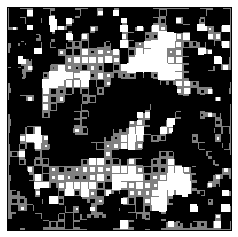
\includegraphics[]{Assets/HINTON1}
  \caption{ Good Hinton Diagram}
  \label{F:TEMP}
  \end{center}
  \end{figure}
  \begin{figure}[]
  \begin{center}
    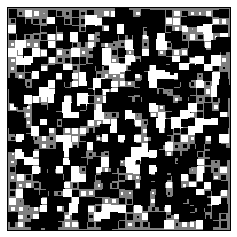
\includegraphics[]{Assets/HINTON2}
  \caption{Bad Hinton Diagram}
  \label{F:TEMP}
  \end{center}
  \end{figure}


  \section{A New Approach - The ORBM}

  \begin{itemize}
    \item Frean and Maslands new approach combines the Restricted Boltzmann Machine and the Sigmoid Belief Network, the RBMs allowing the rich complex causes to be encoded independantly, and the Sigmoid Belief Network modelling the combination of the causes to form the observable data.'
    \item By building on these existing methods can leverage exisitng algorithms
    \item Can verify the inference algorithm with pre trained RBMs for each cause.
    \item Like the RBM leveraged in the ORBM, it is difficult to evaluate, But similar techniques can be leveraged

  \end{itemsize}

  \subsection{Architecture}

  \begin{itemize}
      \item Two RBMs, on for each cause, then they combine via a Sigmoid Beleif Layer. Weights between the RBM and Sigmoid Layers are shared. (TODO-A-DIAGRAM)
      \item Diagram of the ORBM Architecture Including U Layer. Make sure I'm explaining the U layer.
      \item In fact Ua, Ub are like mirrors of the visible.
  \end{itemize}

  \subsection{Inference In the ORBM}

  The difference in architecture from an RBM means that a slightly different inference algorithm is required, as the representations are represented separately for a composite input.

  \begin{itemize}
    \item Inference in this generative model is P(ha, hb given v) , we want to represent the causes separately.

    \item Unfornately, ha and hb are dependant given the visible v. meaning to perform inference, obtaining a hidden representation requires a Gibbs chain
    \item Diagram showing the inference gibbs chain.

  \end{itemize}


  \subsubsection{Calculating the Posterior}

  To find the $ P(h_a, h_b | v_{comp}) $, where $h_a$ and $h_b$ are the separate representations of the data caused $a$ and $b$, and $v_{comp}$ is the composed/composite input. We must sample from a Gibbs Chain,  as $h_a$ and $h_b$ are dependant given $v_{comp}$. This ends up being almost identical to the RBM except we add a 'Correction', when computing the update for $h_a$ and $h_b$ respectively.

  TODO-SHOW-THE-FULL-CORRECTION

  \subsection{Source Separation - Reconstructions in the ORBM}

  To actually perform source separation, one needs to simply take the internal representation generated by the inference step, and generate a visible pattern in the same way you would with a standalone RBM.
